% !TeX encoding = UTF-8
% !TeX spellcheck = en_US

\section{Graph Transformation with eMoflon::IBeX}
	\begin{frame}
		\frametitle{Contents}
		\tableofcontents[currentsection]
	\end{frame}

\subsection{Rule Editor}
	\begin{frame}
		\frametitle{Graph Transformation with eMoflon::IBeX}
		\framesubtitle{Rule Editor: Textual Syntax of Example Rule}
		\begin{center}
			\includegraphics[width=0.65\textwidth]{../common/figures/editor-rule-moveCharacter}
		\end{center}
	\end{frame}
	\begin{frame}
		\frametitle{Graph Transformation with eMoflon::IBeX}
		\framesubtitle{Rule Editor: Visualization}
		\begin{columns}
			\begin{column}{0.5\textwidth}
				\includegraphics[width=\linewidth]{../common/figures/rule-moveCharacter}
			\end{column}
			\begin{column}{0.5\textwidth}
				\includegraphics[width=\linewidth]{../common/figures/rule-moveCharacterToNeighboringPlatform}
			\end{column}
		\end{columns}
	\end{frame}

\subsection{Transform Editor Rules into Patterns}
	\begin{frame}
		\frametitle{Graph Transformation with eMoflon::IBeX}
		\framesubtitle{Transform Editor Rules into Patterns}
		\begin{center}
			\resizebox{!}{0.75\textheight}{
				% !TeX encoding = UTF-8
% !TeX spellcheck = en_US

\begin{tikzpicture} [
		auto,
		node distance = 2.25cm,
		node/.style = {
			rectangle,
			rounded corners,
			thick,
			text width = 6em,
			text centered,
			minimum height = 3em,
		},
		line/.style = {
			draw,
			thick,
			->,
			shorten >=2pt,
		},
		line-caption/.style = {
			font = \footnotesize
		},
		ibex-ui/.style = {
			draw = green!60!lime,
			fill = green!60!lime,
		},
		ibex/.style = {
			draw = blue!20!cyan,
			fill = blue!20!cyan,
		},
		ibex-democles/.style = {
			draw = red!10!orange,
			fill = red!10!orange
		}
	]

	\node[node, ibex-ui] (f) {
		\texttt{gt} text file
	};

	\node[node, ibex-ui, below of = f] (e) {
		Editor Model
	};
	\node[node, ibex-ui, left = 2cm of e] (ev) {
		Editor Model Visualization
	};
	\node[node, ibex-ui, right = 2cm of e] (em) {
		Xtext-based Meta-Model
	};

	\node[node, ibex, below of = e, xshift = 1.6cm] (g) {
		GT API Model
	};
	\node[node, ibex, right = 2cm of g] (gm) {
		GT API Meta-Model
	};
	\node[node, ibex, below of = g] (gc) {
		Java API
	};

	\node[node, ibex, below of = e, xshift = -1.6cm] (i) {
		IBeX Patterns
	};
	\node[node, ibex, left = 2cm of i] (im) {
		IBeX Pattern Meta-Model
	};
	\node[node, ibex, below of = i] (iv) {
		IBeX Pattern Visualization
	};

	\node[node, ibex-democles, below of = im] (d) {
		Democles Patterns
	};
	\node[node, ibex-democles, below of = d] (dm) {
		Democles Meta-Model
	};
	\node[node, ibex-democles, below of = iv] (dv) {
		Democles Visualization
	};

	\begin{scope} [
			every path/.style = line, ibex-ui,
			every node/.style = line-caption
		]
		\path (f) -- node[right] {Xtext transformation} (e);
		\path (e) -- node[below] {visualized in} (ev);
		\path (e) -- node[below] {conforms to} (em);
	\end{scope}

	\begin{scope} [
			every path/.style = line, ibex,
			every node/.style = line-caption
		]
		\path (e) -- node[left, xshift = -0.2cm] {transformation} (i.north);
		\path (e) -- node[right, xshift = 0.2cm] {transformation} (g.north);

		\path (i) -- node[below] {conforms to} (im);
		\path (i) -- node[right] {visualized in} (iv);

		\path (g) -- node[below] {conforms to} (gm);
		\path (g) -- node[right] {code generation} (gc);
	\end{scope}

	\begin{scope} [
			every path/.style = line, ibex-democles,
			every node/.style = line-caption
		]
		\path (i) -- node[left, yshift = 0.2cm] {transformation} (d.east);
		\path (d) -- node[right] {conforms to} (dm);
		\path (d) -- node[right, xshift = 0.2cm] {visualized in} (dv);
	\end{scope}
\end{tikzpicture}

			}
		\end{center}
	\end{frame}

\subsection{Java API}
	\begin{frame}
		\frametitle{Graph Transformation with eMoflon::IBeX}
		\framesubtitle{Java API: Count Matches}
		\includegraphics[width=\textwidth]{../common/code/example-countMatches}
	\end{frame}
	\begin{frame}
		\frametitle{Graph Transformation with eMoflon::IBeX}
		\framesubtitle{Java API: Rule Application}
		\includegraphics[width=\textwidth]{../common/code/example-rule-application}
	\end{frame}
	\begin{frame}
		\frametitle{Graph Transformation with eMoflon::IBeX}
		\framesubtitle{Java API: Subscriptions -- Exploit Incrementality}
		\includegraphics[width=\textwidth]{../common/code/example-subscriptions}
	\end{frame}

\subsection{Integration with the TGG Part}
	\begin{frame}
		\frametitle{Graph Transformation with eMoflon::IBeX}
		\framesubtitle{Integration with the TGG Part}
		\begin{center}
			\resizebox{\linewidth}{!}{
				% !TeX encoding = UTF-8
% !TeX spellcheck = en_US

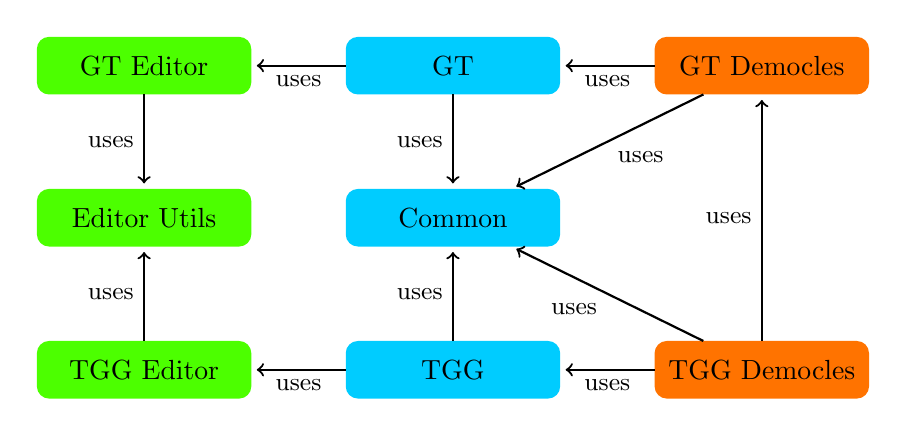
\begin{tikzpicture} [
		auto,
		node/.style = {
			rectangle,
			rounded corners,
			thick,
			text width = 7em,
			text centered,
			minimum height = 2em,
		},
		line/.style = {
			draw,
			thick,
			->,
			shorten >=2pt,
		},
		line-caption/.style = {
			font = \small,
		},
		ibex-ui/.style = {
			draw = green!60!lime,
			fill = green!60!lime,
		},
		ibex/.style = {
			draw = blue!20!cyan,
			fill = blue!20!cyan,
		},
		ibex-democles/.style = {
			draw = red!10!orange,
			fill = red!10!orange
		}
	]

	\matrix[
		column sep = 12mm,
		row sep = 12mm
	] {
		\node[node, ibex-ui] (uiGT) {
			GT Editor
		};
		& \node[node, ibex](GT) {
			GT
		};
		& \node[node, ibex-democles](democlesGT) {
			GT Democles
		};
		\\
		\node[node, ibex-ui] (uiCommon) {
			Editor Utils
		};
		& \node[node, ibex](common) {
			Common
		};
		\\
		\node[node, ibex-ui] (uiTGG) {
			TGG Editor
		};
		& \node[node, ibex](TGG) {
			TGG
		};
		& \node[node, ibex-democles](democlesTGG) {
			TGG Democles
		};
		\\
	};

	\begin{scope} [
		every path/.style = line,
		every node/.style = line-caption
		]
		\path (uiGT) -- node[left] {uses} (uiCommon);
		\path (uiTGG) -- node[left] {uses} (uiCommon);

		\path (GT) -- node {uses} (uiGT);
		\path (TGG) -- node {uses} (uiTGG);

		\path (GT) -- node[left] {uses} (common);
		\path (TGG) -- node[left] {uses} (common);

		\path (democlesGT) -- node {uses} (GT);
		\path (democlesGT) -- node {uses} (common);
		\path (democlesTGG) -- node {uses} (common);
		\path (democlesTGG) -- node {uses} (TGG);
		\path (democlesTGG) -- node {uses} (democlesGT);
	\end{scope}
\end{tikzpicture}

			}
		\end{center}
	\end{frame}
